\section{修正单纯形法}
\label{sec:simplex-revised}

前面把算法写成了矩阵公式，每轮都出现$\bm{A}_B^{-1}$。接下来要弄清：真正计算时应该保存什么，每轮要做多少运算？

\paragraph{完整的单纯形表}
最直接的办法是把所有非基变量的表示都算出来，存成一张表。\term{单纯形表}（simplex tableau）的主体是$\bm{A}_B^{-1}[\bm{b}\ \ \bm{A}]$，再加一行约化成本。例中第$2$轮的基是$(1,4,2)$，表~\ref{tab:simplex-tableau}的上半部分就是这张表，每一列都是对应$\bm{a}_j$在当前基下的表示，$u$和$\bar{x}_B$都可以直接读出。

换基就是对这张表做一次Gauss--Jordan消元，主元取在出基行和入基列的交点。例中主元是$x_4$行$x_5$列的$3$。把该行除以$3$，再用它消去$x_5$列的其他元素，就得到下半部分，也就是第$3$轮的表。

\begin{BookInlineTable}
 \centering
 \begin{tabular}{crrrrrr}
  \toprule
  基 & $\bar{x}$ & $x_1$ & $x_2$ & $x_3$ & $x_4$ & $x_5$\\
  \midrule
  $x_1$ & $2$ & $1$ & $0$ & $1$ & $0$ & $-2$\\
  $x_4$ & $3$ & $0$ & $0$ & $-2$ & $1$ & $3$\\
  $x_2$ & $3$ & $0$ & $1$ & $0$ & $0$ & $1$\\
  $\bm{s}$ & $23$ & $0$ & $0$ & $4$ & $0$ & $-3$\\
  \midrule
  $x_1$ & $4$ & $1$ & $0$ & $-1/3$ & $2/3$ & $0$\\
  $x_5$ & $1$ & $0$ & $0$ & $-2/3$ & $1/3$ & $1$\\
  $x_2$ & $2$ & $0$ & $1$ & $2/3$ & $-1/3$ & $0$\\
  $\bm{s}$ & $26$ & $0$ & $0$ & $2$ & $1$ & $0$\\
  \bottomrule
 \end{tabular}
 \caption{资源配置问题第$2$轮（上）和第$3$轮（下）的单纯形表。第二列是基变量取值，$\bm{s}$行第二列是利润$-f$，其余是约化成本。}
 \label{tab:simplex-tableau}
\end{BookInlineTable}

这张表手算方便，但代价不小：每轮要更新大约$(m+1)(n+1)$个数，无论这一轮用到多少。而且$\bm{A}$稀疏时，$\bm{A}_B^{-1}\bm{A}$通常是稠密的，存储量也不可接受。

\paragraph{每轮真正需要什么}
回头看第~\ref{sec:simplex-basis-exchange}节的计算步骤，一轮只用到四样东西：解一次$\bm{A}_B^\top\bm{y}=\bm{c}_B$，用$\bm{y}$和$\bm{A}$的非基列做内积定价，对入基列解一次$\bm{A}_B\bm{u}=\bm{a}_q$，再做比值检验。表中其他列的表示从未被使用。\term{修正单纯形法}（revised simplex method）因此只维护基矩阵的因子，其余的量需要时再算。一轮的数据流如图~\ref{fig:simplex-revised-flow}所示。

\begin{BookInlineFigure}
 \centering
 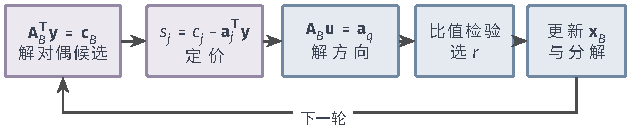
\includegraphics[width=107mm]{figures/05-optimization/01-linear-programming/tikz/simplex-revised-flow/figure.pdf}
 \caption{修正单纯形法一轮的数据流。紫色框处理对偶量：解$\bm{A}_B^\top\bm{y}=\bm{c}_B$得到对偶候选，再对非基列定价。蓝色框处理原始量：解$\bm{A}_B\bm{u}=\bm{a}_q$，比值检验选出基位置，更新基变量和基矩阵的因子。}
 \label{fig:simplex-revised-flow}
\end{BookInlineFigure}

\paragraph{基矩阵逆的更新}
相邻两轮的基矩阵只差一列，无需重新分解。设新基$B'$把第$r$列换成$\bm{a}_q$。由$\bm{a}_q=\bm{A}_B\bm{u}$，新基矩阵可以写成
\[
 \bm{A}_{B'}=\bm{A}_B\bm{F},
\]
其中$\bm{F}$是把单位矩阵第$r$列换成$\bm{u}$的矩阵。两边求逆，只需要$\bm{F}$的逆，它仍是单位矩阵只改第$r$列的形状：
\begin{equation}
 \bm{A}_{B'}^{-1}=\bm{E}\bm{A}_B^{-1},\qquad
 \bm{E}_{:,r}=\bm{\eta},\qquad
 \eta_i=
 \begin{cases}
  -u_i/u_r,& i\neq r,\\
  1/u_r,& i=r.
 \end{cases}
 \label{eq:simplex-eta-update}
\end{equation}
这样的$\bm{E}$只需保存一列，称为eta矩阵。

例中从第$2$轮到第$3$轮，$\bm{u}=(-2,3,1)^\top$，$r=2$，于是
\[
 \bm{E}=\begin{bmatrix}1&2/3&0\\0&1/3&0\\0&-1/3&1\end{bmatrix}.
\]
第$2$轮的基矩阵逆左乘$\bm{E}$，就得到第$3$轮的基矩阵逆：
\begin{equation}
 \bm{A}_{B^{(3)}}^{-1}
 =\bm{E}\begin{bmatrix}1&0&-2\\-2&1&3\\0&0&1\end{bmatrix}
 =\begin{bmatrix}-1/3&2/3&0\\-2/3&1/3&1\\2/3&-1/3&0\end{bmatrix}.
 \label{eq:simplex-final-inverse}
\end{equation}
这个矩阵的第$r$行就是式~\eqref{eq:simplex-row-coefficients}中的$\bm{\rho}$，后两节会反复用到它。

\paragraph{运算量的比较}
表~\ref{tab:simplex-implementation-costs}列出每轮的存储和运算。这里$\operatorname{nnz}(\cdot)$表示非零元个数。修正法的优势在$n\gg m$或$\bm{A}$稀疏时最明显：定价只碰$\bm{A}$的非零元，解方程只碰因子的非零元。

\begin{BookInlineTable}
 \centering
 \begin{tabular}{lll}
  \toprule
  实现方式 & 存储 & 每轮主要运算\\
  \midrule
  完整单纯形表 & $(m+1)(n+1)$ & 约$mn$次更新\\
  修正法，稠密逆 & $m^2$ & 约$m^2+\operatorname{nnz}(\bm{A})$\\
  修正法，LU加eta & 因子的非零元 & 两次三角回代加定价\\
  \bottomrule
 \end{tabular}
 \caption{单纯形法几种实现的每轮代价，均指量级。}
 \label{tab:simplex-implementation-costs}
\end{BookInlineTable}

\paragraph{稀疏性}
大规模问题的基矩阵往往非常稀疏，这时不应显式保存逆。图~\ref{fig:simplex-sparsity}是一个$40$阶三对角矩阵的例子。矩阵本身和它的LU因子都只有$118$个非零位置，而逆矩阵的$1600$个元素全部非零。实际软件保存基矩阵经过行列重排的LU分解，再累积一串eta矩阵，这也是用稀疏因子代替稠密逆的具体办法。重排的目的是减少分解过程中新产生的非零元；LU分解和三角回代的基本算法，可参考\BookChapterRef{chap:direct-linear-solvers}{卷二第12章“线性方程的直接求解”}。

\begin{BookInlineFigure}
 \centering
 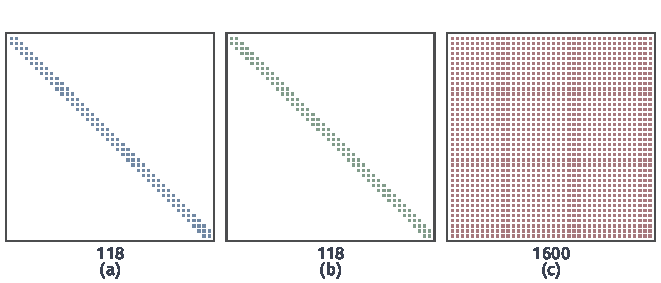
\includegraphics[width=112mm]{figures/05-optimization/01-linear-programming/matplotlib/simplex-sparsity/figure.pdf}
 \caption{$40$阶三对角基矩阵的非零结构，每个小点是一个非零元，图下的数字是非零元总数。(a)~矩阵本身。(b)~不选主元的LU因子合在一起，没有新增非零元。(c)~逆矩阵，全部$1600$个元素非零。}
 \label{fig:simplex-sparsity}
\end{BookInlineFigure}

\paragraph{舍入误差}
连续用eta矩阵更新，每一步都要除以$u_r$。若主元$u_r$很小，比如$10^{-12}$，$\bm{\eta}$的元素可达$10^{12}$量级，舍入误差被同比放大，并一直留在后续的所有计算里。图~\ref{fig:simplex-refactorization}是一个固定随机种子的实验：在$120$阶稠密随机基矩阵上连续换入随机列，比较选取不同主元的残差。总选最大的主元时残差始终在$10^{-13}$左右；总选合格主元中最小的那个时，残差上升好几个数量级，定期重新分解能把它拉回来，但只要继续用小主元，残差又会很快上升。

\begin{BookInlineFigure}
 \centering
 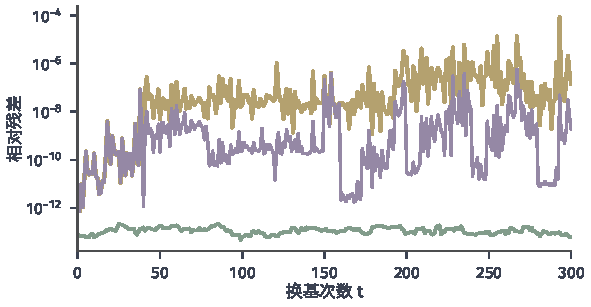
\includegraphics[width=100mm]{figures/05-optimization/01-linear-programming/matplotlib/simplex-refactorization/figure.pdf}
 \caption{用更新后的逆求$\bm{x}_B$时的相对残差$\lVert\bm{A}_B\bm{x}_B-\bm{b}\rVert_2/\lVert\bm{b}\rVert_2$，随机种子固定，矩阵阶数$120$。绿线每步选最大主元且不重分解；黄线每步选$\lvert u_r\rvert>10^{-4}$中最小的主元且不重分解；紫线的选法同黄线，但每$40$次换基重新计算一次逆。}
 \label{fig:simplex-refactorization}
\end{BookInlineFigure}

实验提示了实现时的几条具体做法。比值检验并列或接近并列时，优先选$\lvert u_r\rvert$大的主元，低于主元容差的不选。累积若干个eta矩阵后，重新分解$\bm{A}_B$，用新因子重算$\bm{x}_B,\bm{y},\bm{s}$。

浮点数下的“非负”也只能在容差内判断。常见的可行性容差在$10^{-9}$到$10^{-6}$之间，即接受$x_j\geq-\varepsilon$，约化成本用同样的方式判断。因此算法报告“最优”的含义是：在给定容差下，$\bm{A}\bm{x}=\bm{b}$的残差、$\bm{x}$的负部和$\bm{s}$的负部都足够小。收尾时应该用新的分解重算一遍这三个量，并做必要的尺度还原，因为这些容差是在内部缩放后的问题上判断的，换回原单位后需要另行核查。
